\documentclass[11pt,a4j]{jarticle}
%\usepackage{psfig}
\usepackage[dvipdfmx]{graphicx} % use \includegrahpics
\def\figref#1{図~\ref{#1}}
\def\tabref#1{表~\ref{#1}}
%\def\eqref#1{\ref{#1}~式}
\def\secref#1{\ref{#1}~節}


%%============================================================
%% Layout
%% = = = = = = = = = = = = = = = = = = = = = = = = = = = = = =

\def\setmargin#1#2#3{%	side/top/bottom
	\textwidth = 210mm	%%% Full Size
	\textheight = 296mm	%%% Full Size
	\topmargin = -38mm	%%% 0mm
	\oddsidemargin = -26mm	%%% 0mm
%
	\advance\oddsidemargin + #1
	\evensidemargin = \oddsidemargin
	\advance\textwidth - #1	
	\advance\textwidth - #1
%
	\advance\topmargin + #2
	\advance\textheight - #2 
	\advance\textheight - #3
}

\setmargin{20mm}{25mm}{25mm}


\input{defs.tex}
\iftrue
%\iffalse
\includeonly{
%  ch010_complexGauss
  ch020_entangle
  }
\fi

%\def\ClearPage{\clearpage}
\def\ClearPage{\cleardoublepage}


\begin{document}
%%----------------------------------------------------------------------
\title{Itk::Geo3D Notes}
\author{野田 五十樹}
\date{%
  {\scriptsize
  \begin{tabular}[c]{|l|l|} \hline
  2024/10/04 & 初期バージョン \\ \hline
  2024/10/20 & 屈曲点での円周接続 \\ \hline
 \end{tabular}
  }
}
\maketitle
%% - - - - - - - - - - - - - - - - - - - - - - - - - - - - - - - - - - -
\setcounter{tocdepth}{10}

%\iftrue
\iffalse
\ClearPage
\tableofcontents
\ClearPage\cleardoublepage
\fi
%% - - - - - - - - - - - - - - - - - - - - - - - - - - - - - - - - - - -



%%----------------------------------------------------------------------
\section{class LineSegment}
%% - - - - - - - - - - - - - - - - - - - - - - - - - - - - - - - - - - -

%%--------------------------------------------------
\subsection{closestFractionPairFrom()}
%% - - - - - - - - - - - - - - - - - - - - - - - - -
3次元(以上)の2つの線分の最近点を求める。
求めるものは、各線分上の分率とする。

%%>>>>>>>>>>>>>>>>>>>>>>>>>>>>>>>>>>>>>>>>>>>>>>>>>>
\begin{figure}[h]
  \centering
  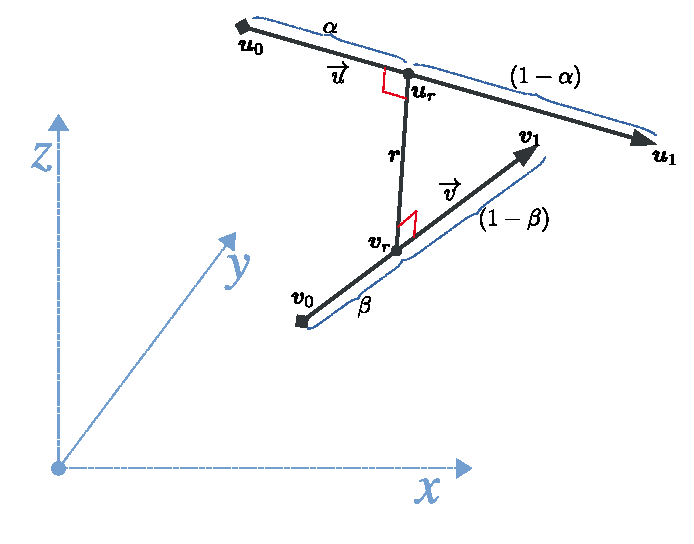
\includegraphics[width=.5\linewidth]{Fig/figure-01.eps}
  \caption{2つの線分の最近距離}
  \label{fig:Fig/figure-01.eps}
\end{figure}
%%>>>>>>>>>>>>>>>>>>>>>>>>>>>>>>>>>>>>>>>>>>>>>>>>>>

まず、2つの線分 $\V{u},\V{v}$ を考える(\figref{fig:Fig/figure-01.eps})。
  %%$$$$$$$$$$$$$$$$$$$$$$$$$$$$$$$$$$$$$$$$
  \begin{eqnarray}
    \V{u} & = & \Tuple{\V{u}_0, \V{u}_1}
  \\
    \V{v} & = & \Tuple{\V{v}_0, \V{v}_1}
  \end{eqnarray}
  %%$$$$$$$$$$$$$$$$$$$$$$$$$$$$$$$$$$$$$$$$
ただし、$ \Tuple{\V{u}_0, \V{u}_1} $ は、
位置 $\V{u}_0$ から位置 $\V{u}_1$ から位置への線分を表す。

線分 $\V{u},\V{v}$ 上の任意の点 $\V{u}_r,\V{u}_r$ は、
その分率を各々 $\alpha,\beta$ として、
次のように表される。
  %%$$$$$$$$$$$$$$$$$$$$$$$$$$$$$$$$$$$$$$$$
  \begin{eqnarray}
    \V{u}_r & = & (1-\alpha) \V{u}_0 + \alpha \V{u}_1
  \\
    \V{v}_r & = & (1-\beta)  \V{v}_0 + \beta  \V{v}_1
  \end{eqnarray}
  %%$$$$$$$$$$$$$$$$$$$$$$$$$$$$$$$$$$$$$$$$
ここで、$\V{r}_u,\V{r}_v$を両端とする線分 $\V{r}$ を考える。
  %%$$$$$$$$$$$$$$$$$$$$$$$$$$$$$$$$$$$$$$$$
  \begin{eqnarray}
    \V{r} & = & \Tuple{\V{u}_r,\V{u}_v}
  \end{eqnarray}
  %%$$$$$$$$$$$$$$$$$$$$$$$$$$$$$$$$$$$$$$$$
また、この線分の方向 $\V{r}_d$ は
  %%$$$$$$$$$$$$$$$$$$$$$$$$$$$$$$$$$$$$$$$$
  \begin{eqnarray}
    \V{r}_d
      & = & \V{v}_r - \V{u}_r
  \\
      & = &
        - \alpha (\V{u}_1 - \V{u}_0)
        + \beta  (\V{v}_1 - \V{v}_0)
        + (\V{v}_0 - \V{u}_0)
  \end{eqnarray}
  %%$$$$$$$$$$$$$$$$$$$$$$$$$$$$$$$$$$$$$$$$

線分 $\V{r}$ が $\V{u},\V{v}$ の最近点を結ぶ線分とすると、
直線 $\V{r}$ と2つの直線 $\V{u},\V{v}$ は互いに直交する。
	\footnote{本来、線分は両端をはみ出さないが、ここでは話を簡単にするため、
	  直線で考える。}
よって、以下の等式が成立する。
  %%$$$$$$$$$$$$$$$$$$$$$$$$$$$$$$$$$$$$$$$$
  \begin{eqnarray}
    (\V{v}_r - \V{u}_r) (\V{u}_1 - \V{u}_0) & = & 0
  \\
    (\V{v}_r - \V{u}_r) (\V{v}_1 - \V{v}_0) & = & 0
  \end{eqnarray}
  %%$$$$$$$$$$$$$$$$$$$$$$$$$$$$$$$$$$$$$$$$
すなわち、
  %%$$$$$$$$$$$$$$$$$$$$$$$$$$$$$$$$$$$$$$$$
  \begin{eqnarray}
    - \alpha (\V{u}_1 - \V{u}_0)^2
    + \beta  (\V{u}_1 - \V{u}_0)(\V{v}_1 - \V{v}_0)
    + (\V{v}_0 - \V{u}_0)(\V{u}_1 - \V{u}_0)
      & = & 0
  \label{eq:r*u}
  \\
    - \alpha (\V{u}_1 - \V{u}_0)(\V{v}_1 - \V{v}_0)
    + \beta  (\V{v}_1 - \V{v}_0)^2
    + (\V{v}_0 - \V{u}_0)(\V{v}_1 - \V{v}_0)
      & = & 0
  \label{eq:r*v}
  \end{eqnarray}
  %%$$$$$$$$$$$$$$$$$$$$$$$$$$$$$$$$$$$$$$$$
ここで、以下の置き換えを行う。
  %%$$$$$$$$$$$$$$$$$$$$$$$$$$$$$$$$$$$$$$$$
  \begin{eqnarray}
    a & = & (\V{u}_1 - \V{u}_0)^2
  \\
    b & = & (\V{v}_1 - \V{v}_0)^2
  \\
    c & = & (\V{u}_1 - \V{u}_0) (\V{v}_1 - \V{v}_0)
  \\
    g & = & (\V{v}_0 - \V{u}_0) (\V{u}_1 - \V{u}_0)
  \\
    h & = & (\V{v}_0 - \V{u}_0) (\V{v}_1 - \V{v}_0)
  \end{eqnarray}
  %%$$$$$$$$$$$$$$$$$$$$$$$$$$$$$$$$$$$$$$$$
これにより、\eqref{eq:r*u},\eqref{eq:r*v}は以下のベクトル式で書ける。
  %%$$$$$$$$$$$$$$$$$$$$$$$$$$$$$$$$$$$$$$$$
  \begin{eqnarray}
    \Mtxx{-a & c \\ -c & b} \Vec{\alpha \\ \beta}
      & = &
        \Vec{-g \\ -h}
  \end{eqnarray}
  %%$$$$$$$$$$$$$$$$$$$$$$$$$$$$$$$$$$$$$$$$
  %%$$$$$$$$$$$$$$$$$$$$$$$$$$$$$$$$$$$$$$$$
  \begin{eqnarray}
    \Vec{\alpha \\ \beta}
      & = &
        \Mtxx{-a & c \\ -c & b}^{-1} 
        \Vec{-g \\ -h}
  \\
      & = &
        \frac{-1}{\det}
        \Mtxx{b & -c \\ c & -a}
        \Vec{g \\ h}
  \end{eqnarray}
  %%$$$$$$$$$$$$$$$$$$$$$$$$$$$$$$$$$$$$$$$$
ただし、$\det$ は上記行列の行列式の値であり、以下の通り。
  %%$$$$$$$$$$$$$$$$$$$$$$$$$$$$$$$$$$$$$$$$
  \begin{eqnarray}
    \det
      & = &
        c^2 - ab
  \end{eqnarray}
  %%$$$$$$$$$$$$$$$$$$$$$$$$$$$$$$$$$$$$$$$$

ここで求まった $\alpha, \beta$ が区間 $[0,1]$ の間であれば、
頂点 $\V{u}_r, \V{v}_r$ は各々、線分 $\V{u}, \V{v}$ 上にある。
それ以外の場合は、直前 $\V{u}, \V{v}$ 上となる。

一方、行列式の値 $\det$ が 0 となるのは、
  %%$$$$$$$$$$$$$$$$$$$$$$$$$$$$$$$$$$$$$$$$
  \begin{eqnarray}
    c^2 - ab
      & = &
        ((\V{u}_1 - \V{u}_0) (\V{v}_1 - \V{v}_0))^2 -
        (\V{u}_1 - \V{u}_0)^2 (\V{v}_1 - \V{v}_0)^2
      = 0
  \\
    ((\V{u}_1 - \V{u}_0) (\V{v}_1 - \V{v}_0))^2
      & = &
        (\V{u}_1 - \V{u}_0)^2 (\V{v}_1 - \V{v}_0)^2
  \\
    (\V{u}_1 - \V{u}_0) (\V{v}_1 - \V{v}_0)
      & = &
        \Abs{\V{u}_1 - \V{u}_0} \Abs{\V{v}_1 - \V{v}_0}
  \end{eqnarray}
  %%$$$$$$$$$$$$$$$$$$$$$$$$$$$$$$$$$$$$$$$$
これは、線分 $\V{u}, \V{v}$ が並行の場合である。
この場合は、$\alpha = \beta = 0$ としてよい。
\footnote{正確には、線分の方向により一方を 1 にする必要がある。}



%%----------------------------------------------------------------------
\section{class Triangle}
%% - - - - - - - - - - - - - - - - - - - - - - - - - - - - - - - - - - -

%%--------------------------------------------------
\subsection{orthogonalDirection()}
%% - - - - - - - - - - - - - - - - - - - - - - - - -
3次元(以上)の空間にある3点 $\V{p}, \V{q}, \V{r}$ で定まる平面$S$の方向 $\V{s}$ を
考える。
ただし、平面$S$の方向とは、平面に対して垂直な方向とする。
また、その平面$S$は原点 $[0,0,0]$ を含まないものとする。
  \footnote{原点を含む場合は、座標系全体を平行移動して原点を含まないようにする。}

%%>>>>>>>>>>>>>>>>>>>>>>>>>>>>>>>>>>>>>>>>>>>>>>>>>>
\begin{figure}[h]
  \centering
  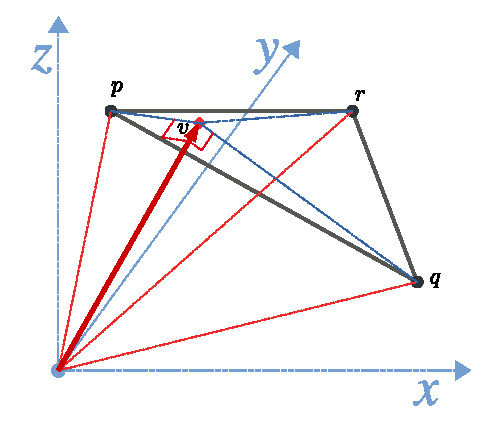
\includegraphics[width=.5\linewidth]{Fig/figure-02.eps}
  \caption{三角形と垂線(法線)}
  \label{fig:Fig/figure-02.eps}
\end{figure}
%%>>>>>>>>>>>>>>>>>>>>>>>>>>>>>>>>>>>>>>>>>>>>>>>>>>

  
平面 $S$ 上の点 $\V{v}$は以下の式で表される。
  %%$$$$$$$$$$$$$$$$$$$$$$$$$$$$$$$$$$$$$$$$
  \begin{eqnarray}
    \V{v}
      & = &
        \alpha \V{p} + \beta \V{q} + (1-\alpha-\beta)\V{r}
  \end{eqnarray}
  %%$$$$$$$$$$$$$$$$$$$$$$$$$$$$$$$$$$$$$$$$
ただし、$\alpha, \beta$ は実数とする。
なお、$\alpha, \beta$ が以下の範囲の時、
$\V{v}$ は三角形 $\Tuple{\V{p},\V{q},\V{r}}$ の内部にある。
  %%$$$$$$$$$$$$$$$$$$$$$$$$$$$$$$$$$$$$$$$$
  \begin{eqnarray}
    & 0 < \alpha < 1
  \\
    & 0 < \beta < 1
  \\
    & 0 < (1-\alpha-\beta) < 1
  \end{eqnarray}
  %%$$$$$$$$$$$$$$$$$$$$$$$$$$$$$$$$$$$$$$$$

ここで、ベクトル $\V{v}$ が平面 $S$ に垂直であるとする。
この場合、以下が成立する。
  %%$$$$$$$$$$$$$$$$$$$$$$$$$$$$$$$$$$$$$$$$
  \begin{eqnarray}
    \V{v} (\V{p} - \V{r}) & = & 0
  \\
    \V{v} (\V{q} - \V{r}) & = & 0
  \end{eqnarray}
  %%$$$$$$$$$$$$$$$$$$$$$$$$$$$$$$$$$$$$$$$$
つまり、
  %%$$$$$$$$$$$$$$$$$$$$$$$$$$$$$$$$$$$$$$$$
  \begin{eqnarray}
      \alpha (\V{p} - \V{r})^2
    + \beta  (\V{q} - \V{r}) (\V{p} - \V{r})
    + \V{r} (\V{p} - \V{r})
      & = & 0
  \label{eq:alpha-qr-beta-qrpr}
  \\
      \alpha (\V{p} - \V{r}) (\V{q} - \V{r})
    + \beta  (\V{p} - \V{r})^2
    + \V{r} (\V{q} - \V{r})
      & = & 0
  \label{eq:alpha-prqr-beta-qr}
  \end{eqnarray}
  %%$$$$$$$$$$$$$$$$$$$$$$$$$$$$$$$$$$$$$$$$
ここで以下の置き換えを行う。
  %%$$$$$$$$$$$$$$$$$$$$$$$$$$$$$$$$$$$$$$$$
  \begin{eqnarray}
    a & = & (\V{p} - \V{r})^2
  \\
    b & = & (\V{p} - \V{r}) (\V{q} - \V{r})
  \\
    c & = & (\V{q} - \V{r})^2
  \\
    g & = & \V{r} (\V{p} - \V{r})
  \\
    h & = & \V{r} (\V{q} - \V{r})
  \end{eqnarray}
  %%$$$$$$$$$$$$$$$$$$$$$$$$$$$$$$$$$$$$$$$$
これにより、\eqref{eq:alpha-qr-beta-qrpr}、\eqref{eq:alpha-prqr-beta-qr}は
以下のように表記できる。
  %%$$$$$$$$$$$$$$$$$$$$$$$$$$$$$$$$$$$$$$$$
  \begin{eqnarray}
    \Mtxx{a & b \\ b & c} \Vec{\alpha \\ \beta}
      & = &
        -\Vec{g \\ h}
  \end{eqnarray}
  %%$$$$$$$$$$$$$$$$$$$$$$$$$$$$$$$$$$$$$$$$
よって、$\alpha, \beta$ は以下の式で求まる。
  %%$$$$$$$$$$$$$$$$$$$$$$$$$$$$$$$$$$$$$$$$
  \begin{eqnarray}
    \Vec{\alpha \\ \beta}
      & = &
        \Mtxx{a & b \\ b & c}^{-1} 
        \left( -\Vec{g \\ h} \right)
  \\
      & = &
        \frac{-1}{\det} \Mtxx{c & -b \\ -b & a}
        \Vec{g \\ h}
  \\
    \det
      & = &
        ac - b^2
  \end{eqnarray}
  %%$$$$$$$$$$$$$$$$$$$$$$$$$$$$$$$$$$$$$$$$
なお、 $\det = 0$ では上記解は求まらない。
これは、$\V{p},\V{q},\V{r}$ の3点の内2つが一致している場合である。


%%--------------------------------------------------
\subsection{orthogonalDirection2()}
%% - - - - - - - - - - - - - - - - - - - - - - - - -
外積の定義より推薦を計算する。

2つのベクトル $\V{u}, \V{v}$ について、以下のような外積 $\V{w}$は、
以下の性質を満たす。
  %%$$$$$$$$$$$$$$$$$$$$$$$$$$$$$$$$$$$$$$$$
  \begin{eqnarray}
    \V{w}
      & = &
        \V{u} \Opd \V{v}
  \\
      & = &
        \Vec{u_y v_z - u_z v_y \\
             u_z v_x - u_x v_z \\
             u_x v_y - u_y v_z}
  \\
    \V{w} \Ipd \V{u}
      & = &
        0
  \\
    \V{w} \Ipd \V{v}
      & = &
        0
  \\
    \Abs{\V{w}}
      & = &
        \mbox{$\V{u}$, $\V{v}$ が張る三角形の面積}
  \end{eqnarray}
  %%$$$$$$$$$$$$$$$$$$$$$$$$$$$$$$$$$$$$$$$$

%%>>>>>>>>>>>>>>>>>>>>>>>>>>>>>>>>>>>>>>>>>>>>>>>>>>
\begin{figure}[h]
  \centering
  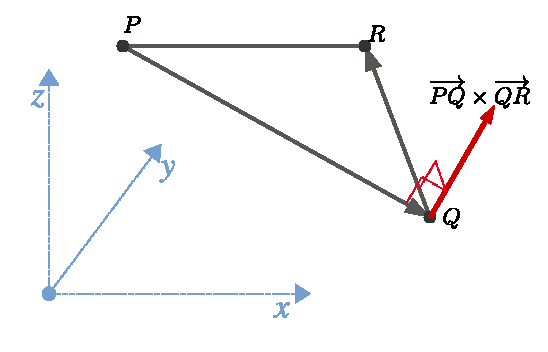
\includegraphics[width=.5\linewidth]{Fig/figure-03.eps}
  \caption{三角形と外積による垂線(法線)}
  \label{fig:Fig/figure-03.eps}
\end{figure}
%%>>>>>>>>>>>>>>>>>>>>>>>>>>>>>>>>>>>>>>>>>>>>>>>>>>

このベクトルの外積を使って、
\figref{fig:Fig/figure-03.eps} のような
三角形 $PQR$ に対する垂線$\V{h}$ は以下のように求めることができる。
 
  %%$$$$$$$$$$$$$$$$$$$$$$$$$$$$$$$$$$$$$$$$
  \begin{eqnarray}
    P: \V{p}
      & = &
        \Tr{\Vec{p_x, p_y, p_z}}
  \\
    Q: \V{q}
      & = &
        \Tr{\Vec{q_x, q_y, q_z}}
  \\
    R: \V{r}
      & = &
        \Tr{\Vec{r_x, r_y, r_z}}
  \end{eqnarray}
  %%$$$$$$$$$$$$$$$$$$$$$$$$$$$$$$$$$$$$$$$$
  \begin{eqnarray}
    \Va{PQ}
      & = &
        \Tr{\Vec{q_x - p_x, q_y - p_y, q_z - p_z}}
  \\
    \Va{QR}
      & = &
        \Tr{\Vec{r_x - q_x, r_y - q_y, r_z - q_z}}
  \end{eqnarray}
  %%$$$$$$$$$$$$$$$$$$$$$$$$$$$$$$$$$$$$$$$$
  \begin{eqnarray}
    \V{h}
      & = &
        \Va{PQ} \Opd \Va{QR}
  \\
      & = &
        \Vec{(q_y - p_y)(r_z - q_z) - (q_z - p_z)(r_y - q_y) \\
             (q_z - p_z)(r_x - q_x) - (q_x - p_x)(r_z - q_z) \\
             (p_x - p_x)(r_y - q_y) - (q_y - p_y)(r_x - q_x)}
  \end{eqnarray}
  %%$$$$$$$$$$$$$$$$$$$$$$$$$$$$$$$$$$$$$$$$

%%--------------------------------------------------
\subsection{屈曲点での半径 $R$ の接続とセットバック}
%% - - - - - - - - - - - - - - - - - - - - - - - - -

%%>>>>>>>>>>>>>>>>>>>>>>>>>>>>>>>>>>>>>>>>>>>>>>>>>>
\begin{figure}[h]
  \centering
  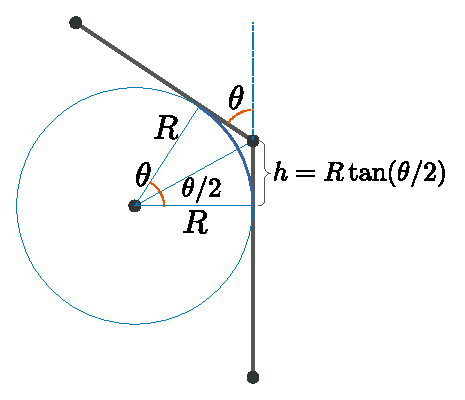
\includegraphics[width=.6\linewidth]{Fig/figure-04.eps}
  \caption{屈曲点での円周に寄る接続とセットバック}
  \label{fig:Fig/figure-04.eps}
\end{figure}
%%>>>>>>>>>>>>>>>>>>>>>>>>>>>>>>>>>>>>>>>>>>>>>>>>>>


2つの連続する線分が角度 $\theta$ をつけて曲がっている時、
その屈曲点で半径 $R$ の円周で接続することを考える。
この場合、円周と線分の接点と屈曲点の間の距離(セットバック)を $h$ とする
(\figref{fig:Fig/figure-04.eps})。

この $h$ は以下の式で表すことができる。
  %%$$$$$$$$$$$$$$$$$$$$$$$$$$$$$$$$$$$$$$$$
  \begin{eqnarray}
    h
      & = &
        R \tan \frac{\theta}{2}
  \end{eqnarray}
  %%$$$$$$$$$$$$$$$$$$$$$$$$$$$$$$$$$$$$$$$$


%%----------------------------------------------------------------------
\section{class Ellipse}
%% - - - - - - - - - - - - - - - - - - - - - - - - - - - - - - - - - - -

%%--------------------------------------------------
\subsection{楕円の定義}
%% - - - - - - - - - - - - - - - - - - - - - - - - -

3次元空間の楕円は、$\Tuple{\V{o}, \V{u}, \V{v}}$ で定義される。
ただし、
  %%$$$$$$$$$$$$$$$$$$$$$$$$$$$$$$$$$$$$$$$$
  \begin{eqnarray}
    \V{o} & : & \mbox{中心}
  \\
    \V{u} & : & \mbox{主軸方向。角度0の方向}
  \\
    \V{v} & : & \mbox{副軸方向。角度90度の方向}
  \end{eqnarray}
  %%$$$$$$$$$$$$$$$$$$$$$$$$$$$$$$$$$$$$$$$$
である。
補助的なパラメータとして、
楕円が属する平面に垂直な方向 $\V{w} $ は、以下を満たす。
  %%$$$$$$$$$$$$$$$$$$$$$$$$$$$$$$$$$$$$$$$$
  \begin{eqnarray}
    \V{u} \cdot \V{w} & = & 0
  \\
    \V{v} \cdot \V{w} & = & 0
  \\
    \V{u} \cdot \V{v} & = & 0
  \end{eqnarray}
  %%$$$$$$$$$$$$$$$$$$$$$$$$$$$$$$$$$$$$$$$$

楕円周上の点 $\V{p}$ と、
その点における接線ベクトル $\dot{\V{p}}$は、
主軸からの角度 $\theta$ をパラメータとして、
  %%$$$$$$$$$$$$$$$$$$$$$$$$$$$$$$$$$$$$$$$$
  \begin{eqnarray}
    \V{p} & = & \V{o} + \cos(\theta) \V{u} + \sin(\theta) \V{v}
  \\
    \dot{\V{p}} & = & - \sin(\theta) \V{u} + \cos(\theta) \V{v}
  \end{eqnarray}
  %%$$$$$$$$$$$$$$$$$$$$$$$$$$$$$$$$$$$$$$$$
で表される。


%%--------------------------------------------------
\subsection{2つの円の最近点}
%% - - - - - - - - - - - - - - - - - - - - - - - - -

%%>>>>>>>>>>>>>>>>>>>>>>>>>>>>>>>>>>>>>>>>>>>>>>>>>>
\begin{figure}[h]
  \centering
  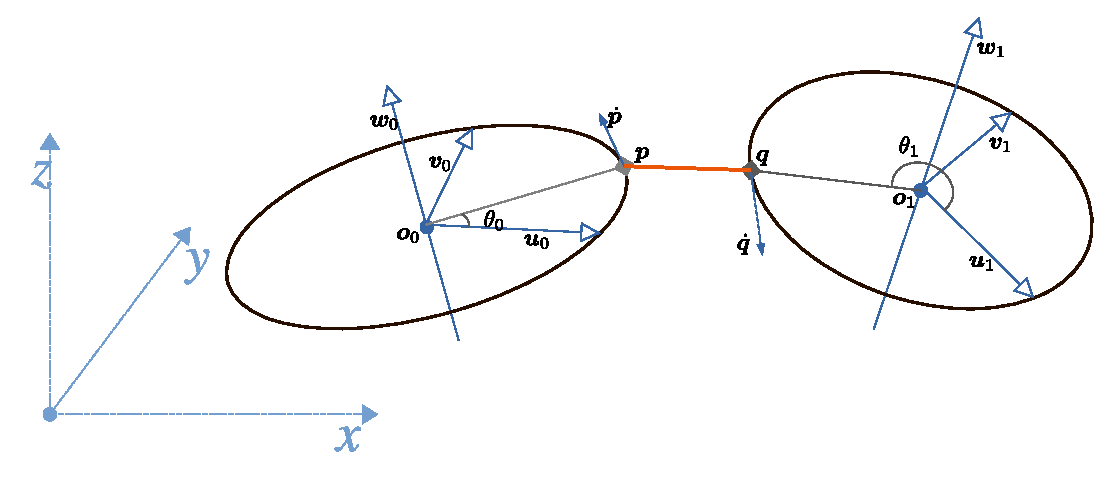
\includegraphics[width=.8\linewidth]{Fig/figure-05.eps}
  \caption{2つの円の最近点}
  \label{fig:Fig/figure-05.eps}
\end{figure}
%%>>>>>>>>>>>>>>>>>>>>>>>>>>>>>>>>>>>>>>>>>>>>>>>>>>

2つの円、
$\Tuple{\V{o}_0, \V{u}_0, \V{v}_0}$、
$\Tuple{\V{o}_1, \V{u}_1, \V{v}_1}$を
考える(\figref{fig:Fig/figure-05.eps})。
この2つの円の最近点を $\V{p}, \V{q}$として、
これらの点の楕円の主軸からの角度を $\theta_0, \theta_1$ としておく。
  %%$$$$$$$$$$$$$$$$$$$$$$$$$$$$$$$$$$$$$$$$
  \begin{eqnarray}
    \V{p} & = & \V{o}_0 + \cos(\theta_0) \V{u}_0 + \sin(\theta_0) \V{v}_0
  \\
    \V{q} & = & \V{o}_1 + \cos(\theta_1) \V{u}_1 + \sin(\theta_1) \V{v}_1
  \\
    \dot{\V{p}} & = & - \sin(\theta_0) \V{u}_0 + \cos(\theta_0) \V{v}_0
  \\
    \dot{\V{q}} & = & - \sin(\theta_1) \V{u}_1 + \cos(\theta_1) \V{v}_1
  \end{eqnarray}
  %%$$$$$$$$$$$$$$$$$$$$$$$$$$$$$$$$$$$$$$$$
さらに、 $\V{p}, \V{q}$ 間のベクトルを $\V{r}$ とする。  
この場合、最近点、すなわち極値であることから以下が成立するはずである。
  %%$$$$$$$$$$$$$$$$$$$$$$$$$$$$$$$$$$$$$$$$
  \begin{eqnarray}
    \V{r} & = & \V{q} - \V{p}
  \\
    \V{r} \cdot \V{w}_0 & = & 0
  \\
    \V{r} \cdot \V{w}_1 & = & 0
  \\
    \V{r} \cdot \dot{\V{p}} & = & 0
  \\
    \V{r} \cdot \dot{\V{q}} & = & 0
  \end{eqnarray}
  %%$$$$$$$$$$$$$$$$$$$$$$$$$$$$$$$$$$$$$$$$

$\V{r}$ を展開すると以下のようになる。
  %%$$$$$$$$$$$$$$$$$$$$$$$$$$$$$$$$$$$$$$$$
  \begin{eqnarray}
    \V{r} = \Vec{r_x \\ r_y \\ r_z}
      & = &
        (\V{o}_1 - \V{o}_0)
      + \Mtxxxx{-\V{u}_0 & -\V{v}_0 & \V{u}_1 & \V{v}_1}
        \Vec{\cos \theta_0 \\
             \sin \theta_0 \\
             \cos \theta_1 \\
             \sin \theta_1}
  \label{eq:r=delta-o-uvuv-cos-sin}
  \end{eqnarray}
  %%$$$$$$$$$$$$$$$$$$$$$$$$$$$$$$$$$$$$$$$$
ここで、以下のように変数を整理する。
  %%$$$$$$$$$$$$$$$$$$$$$$$$$$$$$$$$$$$$$$$$
  \begin{eqnarray}
    \Delta \V{o}
      & = &
        \V{o}_1 - \V{o}_0
  \\
    \M{A}
      & = &
        \Mtxxxx{\V{u}_0 & \V{v}_0 & -\V{u}_1 & -\V{v}_1}
  \\
    \V{\lambda}
      & = &
        \Vec{\cos \theta_0 \\
             \sin \theta_0 \\
             \cos \theta_1 \\
             \sin \theta_1}
  \end{eqnarray}
  %%$$$$$$$$$$$$$$$$$$$$$$$$$$$$$$$$$$$$$$$$
これにより\eqref{eq:r=delta-o-uvuv-cos-sin}は以下になる。
  %%$$$$$$$$$$$$$$$$$$$$$$$$$$$$$$$$$$$$$$$$
  \begin{eqnarray}
    \V{r}
      & = &
        \Delta \V{o} -
        \M{A} \V{\lambda}
  \end{eqnarray}
  %%$$$$$$$$$$$$$$$$$$$$$$$$$$$$$$$$$$$$$$$$
同様に、$\dot{\V{p}}, \dot{\V{q}}$ も以下のように表現する。
  %%$$$$$$$$$$$$$$$$$$$$$$$$$$$$$$$$$$$$$$$$
  \begin{eqnarray}
    \dot{\V{p}}
      & = &
        \Mtxx{\V{v}_0 & -\V{u}_0} \Vec{\cos \theta_0 \\ \sin \theta_0}
  \\
      & = &
        \Mtxxxx{\V{v}_0 & -\V{u}_0 & \V{0} & \V{0}}
        \Vec{\cos \theta_0 \\ \sin \theta_0 \\ \cos \theta_1 \\ \sin \theta_1}
  \\
      & = &
        \M{G} \V{\lambda}
  \end{eqnarray}
  %%$$$$$$$$$$$$$$$$$$$$$$$$$$$$$$$$$$$$$$$$
  %%$$$$$$$$$$$$$$$$$$$$$$$$$$$$$$$$$$$$$$$$
  \begin{eqnarray}
    \dot{\V{q}}
      & = &
        \Mtxx{\V{v}_1 & -\V{u}_1} \Vec{\cos \theta_1 \\ \sin \theta_1}
  \\
      & = &
        \Mtxxxx{\V{0} & \V{0} & \V{v}_1 & -\V{u}_1}
        \Vec{\cos \theta_0 \\ \sin \theta_0 \\ \cos \theta_1 \\ \sin \theta_1}
  \\
      & = &
        \M{H} \V{\lambda}
  \end{eqnarray}
  %%$$$$$$$$$$$$$$$$$$$$$$$$$$$$$$$$$$$$$$$$

よって、整理すると、
  %%$$$$$$$$$$$$$$$$$$$$$$$$$$$$$$$$$$$$$$$$
  \begin{eqnarray}
    \dot{\V{p}} \cdot \V{r}
      & = &
        \Tr{\V{\lambda}}\Tr{\M{G}}
        \left( \Delta \V{o} - \M{A} \V{\lambda} \right) = 0
  \\
    \Tr{\V{\lambda}}\Tr{\M{G}}\Delta\V{o}
      & = &
        \Tr{\V{\lambda}}\Tr{\M{G}}\M{A}\V{\lambda}
  \\
    \dot{\V{q}} \cdot \V{r}
      & = &
        \Tr{\V{\lambda}}\Tr{\M{H}}
        \left( \Delta \V{o} - \M{A} \V{\lambda} \right) = 0
  \\
    \Tr{\V{\lambda}}\Tr{\M{H}}\Delta\V{o}
      & = &
        \Tr{\V{\lambda}}\Tr{\M{H}}\M{A}\V{\lambda}
  \end{eqnarray}
  %%$$$$$$$$$$$$$$$$$$$$$$$$$$$$$$$$$$$$$$$$

つまり、2次形式のベクトル方程式である。

2次形式の方程式を解くためには、
対角化を行えば良い。
つまり、
  %%$$$$$$$$$$$$$$$$$$$$$$$$$$$$$$$$$$$$$$$$
  \begin{eqnarray}
    \Tr{\M{G}} \M{A}
      & = &
        \M{P}^{-1} \M{\Lambda} \M{P}
  \\
    \V{\psi}
      & = &
        \M{P} \V{\lambda}
  \end{eqnarray}
  %%$$$$$$$$$$$$$$$$$$$$$$$$$$$$$$$$$$$$$$$$
とし、
$\M{P}^{-1} = \Tr{\M{P}}$ とすれば、 
  %%$$$$$$$$$$$$$$$$$$$$$$$$$$$$$$$$$$$$$$$$
  \begin{eqnarray}
    \Tr{\V{\lambda}} \Tr{\M{G}} \Delta\V{o}
      & = &
        \Tr{\V{\lambda}} \M{P}^{-1} \M{P} \Tr{\M{G}} \Delta\V{o}
  \\
      & = &
        \Tr{\V{\lambda}} \Tr{\M{P}} \M{P} \Tr{\M{G}} \Delta\V{o}
  \\
      & = &
        \Tr{\V{\psi}} \M{P} \Tr{\M{G}} \Delta\V{o}
  \\
    \Tr{\V{\lambda}}\Tr{\M{G}}\M{A}\V{\lambda}
      & = &
        \Tr{\V{\lambda}}\Tr{\M{P}}\M{\Lambda}\M{P}\V{\lambda}
  \\
      & = &
        \Tr{\V{\psi}} \M{\Lambda} \V{\psi}
  \end{eqnarray}
  %%$$$$$$$$$$$$$$$$$$$$$$$$$$$$$$$$$$$$$$$$
よって、
  %%$$$$$$$$$$$$$$$$$$$$$$$$$$$$$$$$$$$$$$$$
  \begin{eqnarray}
    \Tr{\V{\psi}} \M{P} \Tr{\M{G}} \Delta\V{o}
      & = &
        \Tr{\V{\psi}} \M{\Lambda} \V{\psi}
  \end{eqnarray}
  %%$$$$$$$$$$$$$$$$$$$$$$$$$$$$$$$$$$$$$$$$
これだとなんとか解けそうである。

ただ、以下の難点があり、実際は不可能。
\begin{itemize}
  \item 一般に、$\M{P}^{-1} = \Tr{\M{P}}$ が成り立たない。
      $\M{G}\M{A}$ が対称行列であればよいが、多分違う。
  \item $\M{G}\M{A}$ についても同様の変換が必要であるが、その時の
    変換行列 $\M{P}$ は異なるものとなる。
    異なると、連立で容易には解けなくなる。
\end{itemize}

\end{document}
